%%----------Chapter 2------------------------------------------
\chapter{Background}\label{chap:background}
Measuring the movement of bodies in three dimensional space is not a new field of study.
Especially in our current age of electronics, one can simply grab an accelerometer and microcontroller off of Amazon, have it delivered in 48 hours, and know the experiences felt by a racetrack car or be able to orient a 3D rendering of a bunny \footnote[1]{https://learn.adafruit.com/adafruit-bno055-absolute-orientation-sensor/overview}.
What makes today exciting is that improvements in manufacturing and computational density have drastically increased the capabilities of small embedded systems.
Now, every cell phone has a sophisticated suite of sensors built into them and they have the simple task of detecting whether the phone is in a landscape or portrait mode. 
Some applications, like Google Maps, have gone further and fused the sensor data, along with GPS information, into a robust navigation system.

\section{Inertial Measurement Units} \label{sec:bkg_imu}
Inertial Measurement Units (IMU) are devices that measure the inertial characteristics of a moving body and can report that data to a processor.
The come in a variety of form factors from massive mechanical meters, to microscopic moving machinations.
These sensors come in various grades that each of different use cases and standards associated with them.

The cheapest, least precise, and least accurate IMUs are considered "consumer-grade".
Every day smartphones, cheap commercial breakout boards, and even shipping crates have these devices on-board.
Consumer-grade IMUs can be bought for cents, dollars, or tens of dollars per unit in bulk and are ideal for mass production spaces where quantity is king over quality.
A step up from these sensors are "automotive-grade" IMUs. 
These are tens to hundreds of dollars per unit but are much more accurate and precise than their consumer counter parts.
This makes them desirable for the automotive and industrial sectors as they can assist in automation, control, and monitoring of expensive systems.
The "military-grade" sensors are even more robust and accurate than the previous tiers and have an appropriate military-industrial complex price tag to match. 
These devices will typically be used in applications where friendly war fighters need to know their targets will be impacted or they are going in the right direction in a harsh environment.
Finally, the last major tier is the "navigation-grade" sensors. These sensors are extremely precise, extremely accurate, and cost more than some middle-class families will make in a year.
Primarily, these will be used in survey missions or on underwater vehicles where absolute precision and knowledge of their location is needed.

IMUs are also defined by their measurement Degrees of Freedom (DOF). 
Each measurement axis for each sensor in the IMU contributes a DOF to the sensor.
The common definitions are below in Table \ref{tab:imu_dofs}

\begin{table}[h]
    \caption{Common definitions for IMUs of varying degrees of freedom.}
    \label{tab:imu_dofs}
    \centering
    \begin{tabular}{| c | c | c | c | c |}
        \hline
        DOFs & Accelerometer & Gyroscope & Magnetometer & Barometer \\
        \hline
        3-DOF & 3-axis\footnote[2]{can be either or} & 3-axis\footnote[2] & --- & --- \\
        6-DOF & 3-axis & 3-axis & --- & --- \\
        9-DOF & 3-axis & 3-axis & 3-axis & --- \\
        10-DOF & 3-axis & 3-axis & 3-axis & 1-axis \\
        \hline
    \end{tabular}
\end{table}

\begin{fitbox}[frametitle=Aside: MEMS Technology]
    Test
\end{fitbox}

\subsection{Accelerometer} \label{ssec:bkg_accelerometer}
Accelerometers measure a change in velocity over time (acceleration).
An accelerometer is comprised of a mass suspended in an axis of motion by springs of a known K-constant.
The displacement of the mass along the axis, imparted by a force, is correlated to a sensitivity scale.
Typically, this scale is electrically resistive and creates an analog change in a driving (exciting) voltage.
A basic representation of a three-axis accelerometer is shown in Figure \ref{fig:accelerometers}.

\begin{figure}[h!]
    \caption[Accelerometer block diagram]{Basic block diagram of a three-axis accelerometer where the masses are suspended from springs.}
    \label{fig:accelerometers}
    \centering
    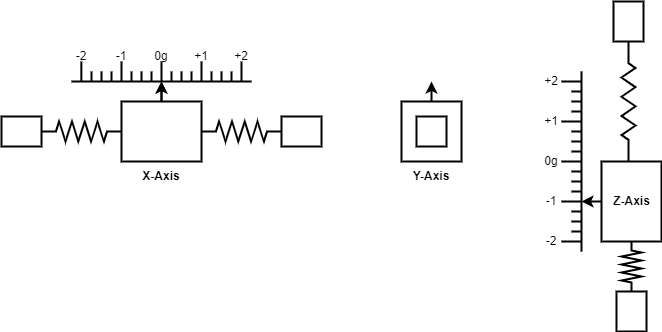
\includegraphics[width=4.5in]{accelerometers.png}
\end{figure}

\subsection{Gyroscope} \label{ssec:bkg_gyroscope}
A gyroscope is an inertial sensor that measures the angular velocity of a rotating body.
MEMS-based gyroscopes measure this value by applying the Coriolis effect on a microscopic mass.

\begin{figure}[h!]
    \caption[Gyroscope block diagram]{Basic block diagram of a three-axis gyroscope where the masses are suspended from springs. The left diagram shows a single mass configuration; the right shows a tuning fork configuration which is twice as sensitive as the singular mass.}
    \label{fig:gyroscopes}
    \centering
    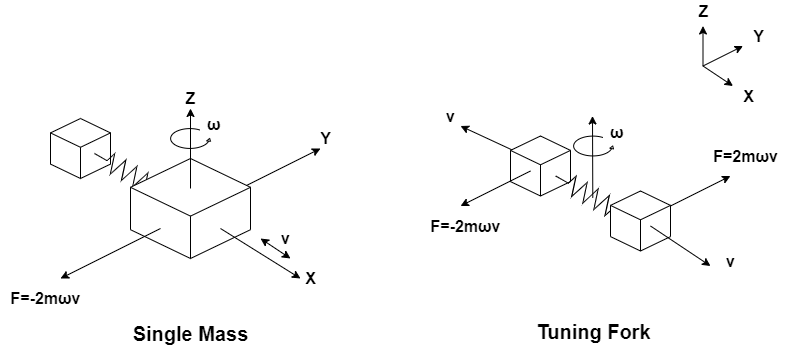
\includegraphics[width=4.5in]{gyroscopes.png}
\end{figure}

As shown in Figure \ref{fig:gyroscopes}, an oscillation is induced on the x-axis using a driving circuit.
While oscillating, if an angular velocity ($\omega$) is imparted on the z-axis, the suspended mass will experience a force in the y-axis that is proportional to $\omega$.
The proof for this relationship can be found in [CITE PROOF].

\subsection{Magnetometer} \label{ssec:bkg_magnetometer}
Magnetometers use magnetoresistive elements that change their effective resistance in the presence of a magnetic field.
Atoms within a magnetoresistive element change their orientations with the magnetic field.
The new orientation can hinder or aid the path of free electrons moving through the element, thus changing the resistance.
By measuring this value and correlating it to a measurement scale, the local magnetic field can be determined.

\begin{figure}[h!]
    \caption[Magnetometer block diagram]{Basic block diagram of a single-axis magnetometer where electrons are flowing through the magnetoresistive material. The left diagram shows the condition when the magnetic field is aligned (minimal resistance); the right shows the non-aligned magnetic field condition which increases the resistance the electrons face passing through the material.}
    \label{fig:magnetometer}
    \centering
    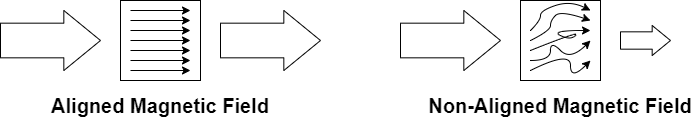
\includegraphics[width=4.5in]{magnetometer.png}
\end{figure}

\section{Global Positioning System} \label{sec:bkg_gps}

\section{Attitude and Heading Reference System} \label{sec:bkg_ahrs}
An Attitude and Heading Reference System (AHRS) is a 6- or 9-DOF IMU equipped with an accelerometer, gyroscope, and/or a magnetometer in all three axes.
The data streams from the sensors can be fused together to estimate a body's inertial orientation in three dimensional space.
The block diagram for this operation is shown in Figure \ref{fig:ahrs_design}.

[INSERT AHRS BLOCK DIAGRAM HERE]

\subsection{Orientation and Rotation} \label{ssec:bkg_orientation}
A body can be rotated in 3D space along the x-, y-, and z-axis.
\textbf{Roll ($\phi$)} defines rotation about the x-axis; \textbf{pitch ($\theta$)} defines rotation about the y-axis; and \textbf{yaw ($\psi$)} defines rotation about the z-axis.
These three rotations are known as Euler angles.
They are easy to conceptually understand and model, but they are not mathematically pure.

[INSERT FIGURE ON BODY ROTATIONS]

A body can be rotated around all three axes to change its orientation and represented as the vector, $<\phi, \theta, \psi>$.
The rotation can occur in a certain sequence, e.g. roll 45 degrees, pitch 45 degrees, then yaw 45 degrees.
This is simple to do so long as two of the rotation axes are not parallel to each other.
When two axes are parallel, they lock together in a condition called, "gimbal lock". 
We can overcome gimbal lock by adding a fourth dimension that can drive each axis independently.
This moves the rotation from the typical three dimensional space to the four dimensional, Hamiltonian, space.
We can represent this orientation as a four dimensional vector called a "quaternion".
This vector is more prevalent in modern AHRS design as it is more mathematically pure and means you do not have to determine if you need to change a rotation sequence to avoid or get out of gimbal lock.

It is possible to freely switch between Euler and quaternion vectors using trigonometric operations inside of a matrix multiplication operation.

\begin{fitbox}[frametitle=Aside: Gimbal Lock]
    When two axes become parallel, eulerian changes to either axis become irrelevant, ergo, the system loses a degree of freedom.
    When in gimbal lock, rotations and plotting yield discontinuities that need to be mitigated by changing the rotation order, or moving two or three axes at once.
    This can create stange pathways for the body and cause unexpected behavior.
    
    The figure below shows a body's rotation while in gimbal lock. The rotation order is roll, pitch, then yaw.
    First, it is pitched 90 degrees upwards to align the roll and yaw axes, $<0, 90, 0>$.
    If we then want to rotate it such that it's orientation is $<90, 0, 0>$, it would be rolled left 90 degrees and pitched down 90 degrees.
    However, due to gimbal lock, the body ended up in the orientation $<0, 0, 90>$!
    To break the gimbal lock and get to the correct orientation, the rotation order would have to be changed to pitch, yaw, roll, or the roll and yaw axes driven simultaneously.
    
    [INSERT FIGURE ON GIMBAL LOCK]
\end{fitbox}

\section{Filters} \label{sec:bkg_filters}
